% =============================================================================
%  CSE 4305 — Computer Organization and Architecture : Assignment 2
%  Simulating a Simple Cache Controller FSM
%  Kanetah Khan  —  230041156
% =============================================================================
\documentclass[11pt,a4paper]{article}

% ---------------- Packages ----------------
\usepackage[margin=1in]{geometry}
\usepackage{amsmath,amssymb}
\usepackage{booktabs}
\usepackage{array}
\usepackage{tabularx}
\usepackage{graphicx}
\usepackage{xcolor}
\usepackage{listings}
\usepackage{hyperref}
\usepackage{tikz}
\usepackage{caption}
\usepackage{titlesec}
\usepackage{fancyhdr}
\usepackage{enumitem}
\usetikzlibrary{positioning,arrows.meta,shapes.geometric,fit,calc}

\hypersetup{
    colorlinks=true,
    linkcolor=black,
    urlcolor=blue,
    citecolor=blue,
}

% ---------------- Code listing style ----------------
\definecolor{codegray}{RGB}{245,245,245}
\definecolor{codekey}{RGB}{0,80,160}
\definecolor{codecomment}{RGB}{120,120,120}
\definecolor{codestr}{RGB}{160,60,60}

\lstdefinestyle{py}{
    language=Python,
    backgroundcolor=\color{codegray},
    basicstyle=\ttfamily\footnotesize,
    keywordstyle=\color{codekey}\bfseries,
    commentstyle=\color{codecomment}\itshape,
    stringstyle=\color{codestr},
    numbers=left,
    numberstyle=\tiny\color{gray},
    numbersep=8pt,
    frame=single,
    rulecolor=\color{gray!40},
    breaklines=true,
    tabsize=2,
    showstringspaces=false,
    captionpos=b,
    xleftmargin=12pt,
}

\lstdefinestyle{trace}{
    backgroundcolor=\color{codegray},
    basicstyle=\ttfamily\scriptsize,
    frame=single,
    rulecolor=\color{gray!40},
    breaklines=false,
    tabsize=2,
    showstringspaces=false,
    xleftmargin=6pt,
    columns=fullflexible,
    keepspaces=true,
}

\lstset{style=py}

% ---------------- Section formatting ----------------
\titleformat{\section}{\Large\bfseries}{\thesection}{0.7em}{}
\titleformat{\subsection}{\large\bfseries}{\thesubsection}{0.6em}{}

\pagestyle{fancy}
\fancyhf{}
\fancyhead[L]{\small CSE 4305 — Assignment 2}
\fancyhead[R]{\small Kanetah Khan (230041156)}
\fancyfoot[C]{\thepage}

% =============================================================================
\begin{document}
% =============================================================================

% ---------------- Cover page ----------------
\begin{titlepage}
    \centering
    \vspace*{1cm}
    {\Large\bfseries Islamic University of Technology\par}
    \vspace{0.3cm}
    {\large Department of Computer Science and Engineering\par}
    \vspace{1.4cm}
    {\itshape CSE 4305 — Computer Organization and Architecture\par}
    \vspace{0.3cm}
    {\large Assignment 2\par}
    \vspace{1.6cm}
    \rule{\linewidth}{0.5pt}
    \vspace{0.3cm}

    {\Huge\bfseries Simulating a Simple\\[0.3em]
     Cache Controller FSM\par}
    \vspace{0.3cm}
    \rule{\linewidth}{0.5pt}

    \vspace{2.2cm}
    {\bfseries Submitted by:\par}
    \vspace{0.6cm}
    \begin{tabular}{rl}
        \textit{Name}        & : \textbf{Kanetah Khan} \\
        \textit{Student ID}  & : \textbf{230041156} \\
        \textit{Programme}   & : B.Sc. in Computer Science and Engineering \\
        \textit{Semester}    & : 3rd Semester, Group B \\
    \end{tabular}

    \vspace{1.6cm}
    {\bfseries Submitted to:\par}
    \vspace{0.4cm}
    Mohammad Ishrak Abedin\\
    Lecturer, Department of CSE

    \vfill
    \textbf{Submission Date:} 16\textsuperscript{th} April, 2026\\[0.3em]
    {\small Source repository: \href{https://github.com/KanetahKhan/COA_CSE4305}{%
     \texttt{github.com/KanetahKhan/COA\_CSE4305}}}
\end{titlepage}

% ---------------- TOC ----------------
\tableofcontents
\newpage

% =============================================================================
\section{Introduction}
% =============================================================================

A cache controller is the glue logic that sits between a CPU and main memory,
deciding on every access whether the word being requested is already stored in
the cache or must be fetched from (or written back to) memory. In hardware this
logic is described very cleanly as a \textbf{finite state machine (FSM)}: the
controller is always in exactly one state, and it transitions according to the
CPU request and the response from memory. Patterson and Hennessy
(\textit{Computer Organization and Design: The Hardware/Software Interface,
RISC-V Edition}, \S5.9) describe a textbook cache controller as a four-state
FSM: an idle state, a tag-compare state, a write-back state and an allocate
state. This assignment builds a working cycle-accurate simulator of exactly
such an FSM and verifies, using six carefully chosen read/write traces, that
it behaves the way the textbook describes.

\subsection{Assignment Context and Scope}

The assignment brief asks for a simulator of an FSM-based cache controller
with a simple CPU that only issues read/write requests or waits for a response,
and a simple memory that never misses but has multi-cycle latency. The FSM is
to follow the book's specification (\S5.9), and the report is to describe the
simulator setup, the FSM implementation, and a series of inputs that cover all
the functionalities with their corresponding outputs.

The baseline cache configuration follows the textbook: a direct-mapped cache
with \textbf{8 lines}, a block size of \textbf{4 words}, \textbf{16-bit
addresses}, \textbf{write-back} update policy, and \textbf{write-allocate} on
a write miss.

\subsection{Extensions Beyond the Baseline}

Alongside the required four-state FSM, the submitted simulator adds three
features that are each introduced in Patterson \& Hennessy as standard
optimisations to the textbook cache. They are all implemented, tested and
discussed in this report:

\begin{itemize}[leftmargin=1.4em,itemsep=0.15em]
    \item \textbf{Multi-level memory hierarchy (L1 + L2)} — an L2 cache sits
    between the L1 controller and main memory, with its own tag array,
    replacement policy and access latency. An L2 hit avoids paying the full
    main-memory round-trip.
    \item \textbf{Write-Through / No-Write-Allocate policies} — selectable at
    construction time and covered in \S5.3 of the textbook. A fifth FSM state
    \texttt{WRITE\_THROUGH} handles the case where the write buffer is
    temporarily full.
    \item \textbf{Victim cache} — a small fully-associative FIFO buffer that
    catches recently evicted L1 blocks. On a conflict miss the victim cache is
    consulted first, which can service the access without going to L2 or main
    memory at all.
\end{itemize}

\subsection{What This Report Covers}

Section~\ref{sec:arch} lays out the overall architecture and how the
components are wired together. Section~\ref{sec:cfg} explains the cache
configuration and address decomposition. Section~\ref{sec:fsm} is the core of
the report: it walks through each FSM state and gives the exact transition
conditions. Section~\ref{sec:hier} describes the multi-level L1+L2 memory
hierarchy. Section~\ref{sec:policies} covers the write-through, no-write-allocate
and victim-cache extensions. Section~\ref{sec:sig} catalogues the interfacing
signals. Section~\ref{sec:impl} is a brief tour of the code organisation.
Section~\ref{sec:tests} presents six scenarios with their cycle-by-cycle
simulator output. Section~\ref{sec:perf} collects the performance numbers.
Sections~\ref{sec:build} and \ref{sec:conc} finish with build instructions and
a conclusion.

% =============================================================================
\section{Simulator Architecture}\label{sec:arch}
% =============================================================================

The simulator is organised as three cooperating objects that are ticked once
per simulated clock cycle, exactly mirroring the hardware they represent.
Figure~\ref{fig:blockdiag} shows the top-level block diagram.

\begin{figure}[h]
    \centering
    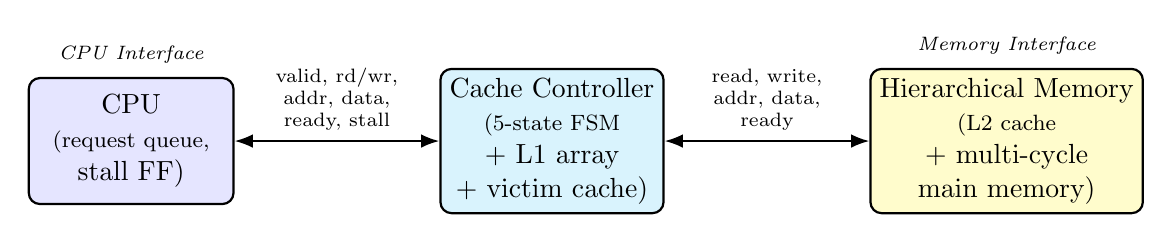
\begin{tikzpicture}[
        node distance=1.8cm,
        box/.style={draw, rounded corners, minimum width=2.6cm, minimum height=1.6cm,
                    align=center, thick},
        iface/.style={<->, >=Latex, thick},
    ]
        \node[box, fill=blue!10] (cpu) {CPU\\\footnotesize(request queue,\\ stall FF)};
        \node[box, fill=cyan!15, right=2.6cm of cpu] (ctrl) {Cache Controller\\\footnotesize(5-state FSM\\+ L1 array\\+ victim cache)};
        \node[box, fill=yellow!20, right=2.6cm of ctrl] (mem) {Hierarchical Memory\\\footnotesize(L2 cache\\+ multi-cycle\\ main memory)};

        \draw[iface] (cpu) -- node[above,font=\scriptsize, align=center]
            {valid, rd/wr,\\ addr, data,\\ ready, stall} (ctrl);
        \draw[iface] (ctrl) -- node[above,font=\scriptsize, align=center]
            {read, write,\\ addr, data,\\ ready} (mem);

        \node[above=0.05cm of cpu, font=\scriptsize\itshape] {CPU Interface};
        \node[above=0.05cm of mem, font=\scriptsize\itshape] {Memory Interface};
    \end{tikzpicture}
    \caption{Top-level block diagram. The three objects exchange state through
    two signal bundles; every bundle is refreshed every clock cycle. The
    hierarchical memory on the right internally contains the L2 cache and
    main-memory model.}
    \label{fig:blockdiag}
\end{figure}

\subsection{The Three Objects}

\textbf{CPU.} The \texttt{CPU} class (file \texttt{cpu.py}) holds an ordered
list of pending requests, each a tuple \texttt{(type, address, data)}. On
every tick it either takes the next request off the queue and forwards it to
the controller, or, if it is still waiting for a result, counts a busy cycle.
When the controller asserts \texttt{ready}, the CPU latches the returned data
and advances to the next request. This mirrors a real pipelined CPU that
stalls the memory stage whenever a cache access takes more than one cycle.

\textbf{Cache controller.} The \texttt{CacheController} class
(file \texttt{cache\_controller.py}) is the heart of the simulator. It owns
the L1 cache array, the FSM state variable, the victim cache, and both
interface signal bundles. Its \texttt{tick()} method dispatches into one of
five state handlers and appends a structured log entry so that the trace can
be reconstructed afterwards.

\textbf{Memory.} Two memory models live in \texttt{memory.py}:
\texttt{Memory} is the basic multi-cycle main memory required by the
assignment, and \texttt{HierarchicalMemory} wraps \texttt{Memory} with an L2
cache between L1 and DRAM. The simulator uses \texttt{HierarchicalMemory} by
default; passing \texttt{enable\_l2=False} falls back to the basic single-level
memory. Both models expose the same signal bundle so the controller cannot
tell which is connected.

\subsection{Simulation Loop}

The \texttt{Simulator} class (file \texttt{simulator.py}) ties the three
objects together. Its run loop is, in essence,

\begin{lstlisting}
while not self.cpu.is_done():
    new_req = self.cpu.tick(ctrl.cpu.ready, ctrl.cpu.data_out)
    if new_req:
        ctrl.submit_request(*new_req)
    self.memory.tick()                          # L2 / main-memory state
    ctrl.mem.ready   = self.memory.ready
    ctrl.mem.data_in = self.memory.buffer
    ctrl.set_write_buffer_status(wb_has_room)   # back-pressure to FSM
    ctrl.tick()                                 # FSM advances one step

    if ctrl.state == ALLOCATE and not memory.busy:
        self.memory.start_read(ctrl.mem.address)
    elif write_buffer_has_entry and not memory.busy:
        self.memory.start_write(...)
\end{lstlisting}

Each pass through the loop is one clock cycle. Memory is ticked \emph{before}
the controller so that a memory \texttt{ready} signal produced this cycle is
visible to the controller in the same cycle — matching synchronous digital
logic where the memory's output registers are sampled on the rising edge.
After the controller ticks, the simulator starts a new memory transaction if
the controller has just entered \texttt{ALLOCATE}, or drains a queued write
from the write buffer if the memory bus is free.

% =============================================================================
\section{Cache Configuration and Address Decomposition}\label{sec:cfg}
% =============================================================================

The baseline configuration used in Tests 1–5 is a direct-mapped cache with
\textbf{8 lines, block size of 4 words, 16-bit addresses, main-memory read
latency of 3 cycles and main-memory write latency of 2 cycles}, with an L2
cache of \textbf{16 lines at 2-cycle latency}. Test 6 shrinks L1 to 4 lines
and increases main-memory latencies. Table~\ref{tab:cfg} summarises the
parameters.

\begin{table}[h]
    \centering
    \caption{Cache and memory configuration.}
    \label{tab:cfg}
    \begin{tabular}{@{}lll@{}}
        \toprule
        \textbf{Parameter} & \textbf{Default (Tests 1–5)} & \textbf{Test 6 (stress)} \\
        \midrule
        L1 cache lines          & 8                  & 4 \\
        L1 associativity        & 1 (Direct-Mapped)  & 1 (Direct-Mapped) \\
        Block size              & 4 words            & 4 words \\
        Address width           & 16 bits            & 16 bits \\
        L2 cache lines          & 16                 & 16 \\
        L2 latency              & 2 cycles           & 2 cycles \\
        Main-memory read lat.   & 3 cycles           & 4 cycles \\
        Main-memory write lat.  & 2 cycles           & 3 cycles \\
        Write-hit policy        & Write-Back         & Write-Back \\
        Write-miss policy       & Write-Allocate     & Write-Allocate \\
        Write-buffer size       & 4 entries          & 4 entries \\
        \bottomrule
    \end{tabular}
\end{table}

\subsection{Address Decomposition}

Every incoming address is split into three fields by the controller's
\texttt{\_decompose\_address} helper:

\begin{itemize}[leftmargin=1.4em,itemsep=0.1em]
    \item \textbf{Offset} — low-order bits that pick a word within a block.
    With block size 4, offset $= \lceil \log_2 4 \rceil = 2$ bits.
    \item \textbf{Index} — next bits that pick a set. With 8 sets,
    index $= \lceil \log_2 8 \rceil = 3$ bits.
    \item \textbf{Tag} — the remaining high-order bits. With 16-bit addresses,
    $\text{tag} = 16 - 3 - 2 = 11$ bits.
\end{itemize}

Figure~\ref{fig:addr} shows the layout. The four-line stress configuration in
Test 6 uses offset = 2, index = 2, tag = 12.

\begin{figure}[h]
    \centering
    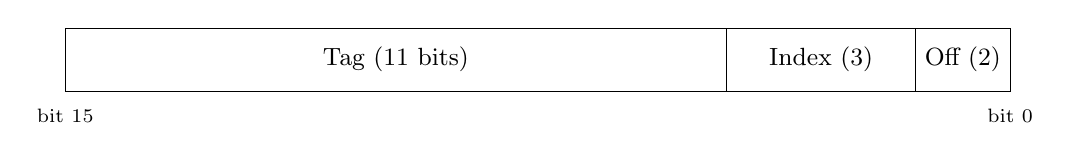
\begin{tikzpicture}[every node/.style={font=\small}]
        \draw (0,0) rectangle (12,0.8);
        \draw (8.4,0) -- (8.4,0.8);
        \draw (10.8,0) -- (10.8,0.8);
        \node at (4.2,0.4) {Tag (11 bits)};
        \node at (9.6,0.4) {Index (3)};
        \node at (11.4,0.4) {Off (2)};
        \node[below=0.1cm] at (0,0) {\scriptsize bit 15};
        \node[below=0.1cm] at (12,0) {\scriptsize bit 0};
    \end{tikzpicture}
    \caption{Address decomposition for the 16-bit, 8-line, 4-word-block
    baseline configuration.}
    \label{fig:addr}
\end{figure}

\subsection{Cache Line Structure}

Each L1 cache line stores a valid bit, a dirty bit, the tag, and the block of
4 data words. Two extra fields (\texttt{lru\_counter} and
\texttt{access\_count}) are included so that set-associative configurations
can support LRU and LFU replacement without changing the data structure:

\begin{lstlisting}
@dataclass
class CacheLine:
    valid:        bool = False
    dirty:        bool = False
    tag:          int  = 0
    data:         list = field(default_factory=lambda: [0] * 4)
    lru_counter:  int  = 0   # timestamp of last access (LRU)
    access_count: int  = 0   # total accesses (LFU)
    write_count:  int  = 0   # dirty writes to this line
\end{lstlisting}

The valid bit distinguishes a cold (empty) line from one that has ever been
filled; the dirty bit records that a write-hit has modified the line but the
change has not yet propagated to memory. Together these two bits control the
branching in the \texttt{COMPARE\_TAG} state.

% =============================================================================
\section{Finite State Machine Design}\label{sec:fsm}
% =============================================================================

The controller is a Moore machine: the outputs (CPU stall/ready and memory
read/write) are a function of the current state and the saved request, not of
the raw inputs. Figure~\ref{fig:fsm} is the full state diagram. Four states
come directly from Patterson \& Hennessy \S5.9 (\texttt{IDLE},
\texttt{COMPARE\_TAG}, \texttt{WRITE\_BACK}, \texttt{ALLOCATE}). A fifth
state, \texttt{WRITE\_THROUGH}, handles a deferred write-through when the
write buffer has run out of room (see \S\ref{sec:policies}).

\begin{figure}[h]
    \centering
    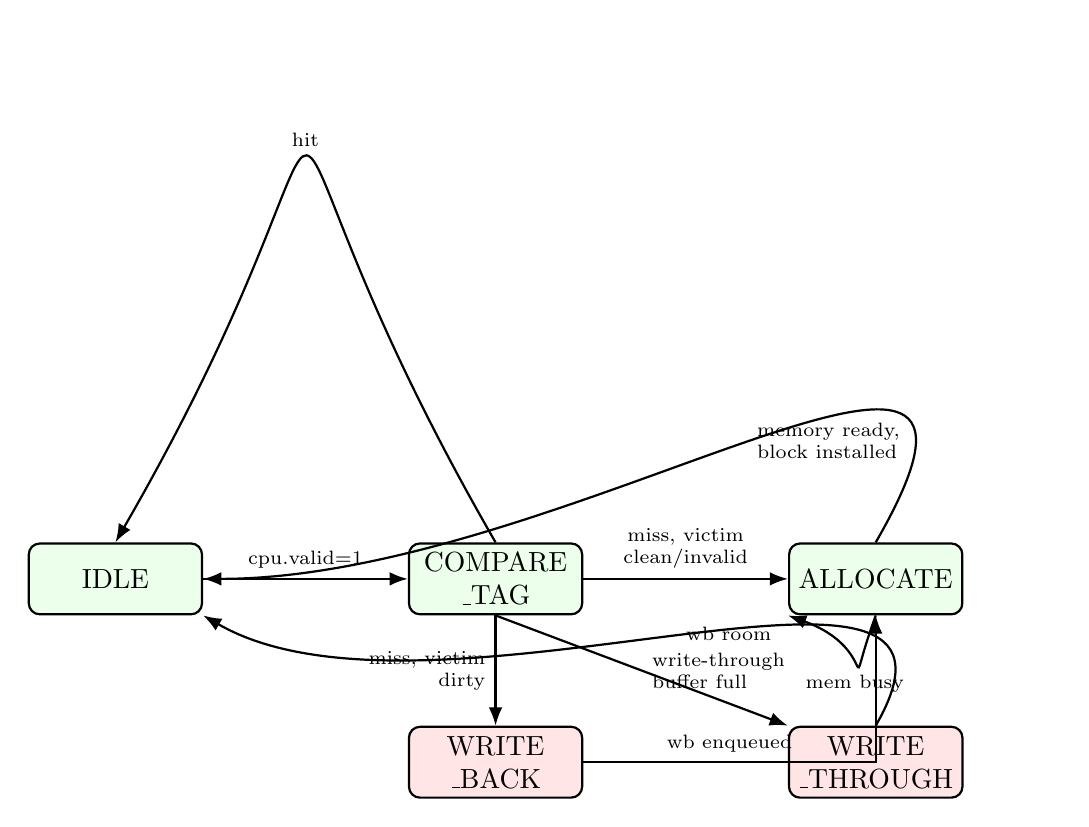
\begin{tikzpicture}[
        node distance=2.2cm and 2.6cm,
        state/.style={draw, rounded corners, minimum width=2.2cm, minimum height=0.9cm,
                      align=center, thick, fill=green!8},
        busy/.style={state, fill=red!10},
        arrow/.style={->, >=Latex, thick},
    ]
        \node[state]                         (idle)  {IDLE};
        \node[state, right=of idle]          (cmp)   {COMPARE\\\_TAG};
        \node[state, right=of cmp]           (alloc) {ALLOCATE};
        \node[busy, below=1.4cm of cmp]      (wb)    {WRITE\\\_BACK};
        \node[busy, below=1.4cm of alloc]    (wt)    {WRITE\\\_THROUGH};

        \draw[arrow] (idle)  -- node[above,font=\scriptsize] {cpu.valid=1} (cmp);
        \draw[arrow] (cmp.north) to [out=120,in=60,looseness=4]
            node[above,font=\scriptsize] {hit} (idle.north);
        \draw[arrow] (cmp)   -- node[above,font=\scriptsize,align=center]
            {miss, victim\\ clean/invalid} (alloc);
        \draw[arrow] (cmp)   -- node[left,font=\scriptsize,align=right]
            {miss, victim\\ dirty} (wb);
        \draw[arrow] (wb)    -| node[pos=0.25,above,font=\scriptsize] {wb enqueued} (alloc);
        \draw[arrow] (alloc.north) to [out=60,in=0,looseness=1.4]
            node[right,font=\scriptsize,align=left] {memory ready,\\block installed} (idle.east);
        \draw[arrow] (alloc.south) to [out=-110,in=-20,looseness=3]
            node[below,font=\scriptsize] {mem busy} (alloc.south west);
        \draw[arrow] (cmp.south) -- node[right,font=\scriptsize,align=left]
            {write-through\\ buffer full} (wt.north west);
        \draw[arrow] (wt.north) to [out=60,in=-30]
            node[right,font=\scriptsize] {wb room} (idle.south east);
    \end{tikzpicture}
    \caption{Five-state FSM. The four core states (IDLE, COMPARE\_TAG,
    WRITE\_BACK, ALLOCATE) come from Patterson \& Hennessy \S5.9. The
    WRITE\_THROUGH state is added to stall a write-through when the write
    buffer is temporarily full; it is only reached when
    \texttt{write\_policy = Write-Through}.}
    \label{fig:fsm}
\end{figure}

\subsection{State IDLE}

In this state the controller is waiting. CPU \texttt{stall} is low (the CPU
is free to fetch its next instruction) and both \texttt{mem.read} and
\texttt{mem.write} are low (the memory bus is idle). On every rising edge the
controller checks \texttt{cpu.valid}: if it is asserted, the controller
latches the incoming request (\texttt{saved\_request}, \texttt{saved\_address},
\texttt{saved\_data}), raises \texttt{stall}, and transitions to
\texttt{COMPARE\_TAG} on the next cycle.

\begin{lstlisting}
def _handle_idle(self):
    if self.cpu.valid:
        self.saved_address = self.cpu.address
        self.saved_request = self.cpu.read_write
        self.saved_data    = self.cpu.data_in
        self.cpu.stall     = True
        self.state         = State.COMPARE_TAG
\end{lstlisting}

\subsection{State COMPARE\_TAG}

This is a single-cycle state in which the saved address is split into
tag/index/offset, the cache line at that index is looked up, and one of four
things happens:

\begin{enumerate}[leftmargin=1.4em,itemsep=0.15em]
    \item \textbf{Read hit.} The stored tag matches and the line is valid.
    The word at the computed offset is driven onto \texttt{cpu.data\_out},
    \texttt{cpu.ready} is raised for one cycle, and the FSM returns to
    \texttt{IDLE}.
    \item \textbf{Write hit.} Same tag match, but the saved data word is
    written into the block at the computed offset. The line's dirty bit is
    set; \texttt{cpu.ready} is raised and the FSM returns to \texttt{IDLE}.
    \item \textbf{Miss, victim clean or invalid.} Tag mismatch (or cold
    line). The FSM transitions directly to \texttt{ALLOCATE} so the correct
    block can be fetched; no write-back is required.
    \item \textbf{Miss, victim dirty.} Tag mismatch and the current occupant
    has been modified. The block has to be written back to memory before it
    is overwritten, so the FSM transitions to \texttt{WRITE\_BACK}.
\end{enumerate}

When the victim cache is enabled, it is consulted between steps 2 and 3/4;
a victim-cache hit short-circuits the miss handling and the FSM returns to
\texttt{IDLE} directly (see \S\ref{sec:policies}).

\begin{lstlisting}
def _handle_compare_tag(self):
    tag, set_idx, offset = self._decompose_address(self.saved_address)
    hit_way = self._find_hit_way(set_idx, tag)

    if hit_way >= 0:
        line = self.cache[set_idx][hit_way]
        self._touch(set_idx, hit_way)
        if self.saved_request == RequestType.READ:
            self.cpu.data_out = line.data[offset]
        else:
            line.data[offset] = self.saved_data
            line.dirty = True
        self.cpu.ready = True
        self.state     = State.IDLE
    else:
        victim_way  = self._find_victim_way(set_idx)
        victim_line = self.cache[set_idx][victim_way]
        if self._try_victim_swap(tag, set_idx, victim_way, offset):
            return
        if victim_line.valid and victim_line.dirty:
            self.state = State.WRITE_BACK
        else:
            self.state = State.ALLOCATE
\end{lstlisting}

\subsection{State WRITE\_BACK}

The controller enqueues the entire dirty block into a small write buffer so
that the subsequent \texttt{ALLOCATE} can proceed in parallel with the memory
write. Enqueuing takes one cycle — after which the controller transitions to
\texttt{ALLOCATE}. The buffered block is drained to memory by the simulator
as soon as the memory bus becomes free. This matches the textbook's
recommendation of using a write buffer to overlap the write-back with the
fetch.

\begin{lstlisting}
def _handle_write_back(self):
    set_idx, way = self.saved_set, self.saved_way
    line = self.cache[set_idx][way]
    wb_addr = self._block_address(line.tag, set_idx)
    self._pending_writeback_enqueue = {
        "address": wb_addr,
        "data":    list(line.data),
    }
    line.dirty = False
    self.state = State.ALLOCATE
\end{lstlisting}

\subsection{State ALLOCATE}

The controller asserts \texttt{mem.read} with the block-aligned address of
the requested block and counts cycles while memory responds. When
\texttt{mem.ready} is finally asserted, the fetched block is installed into
the victim way, the valid bit is set, and then the original CPU request is
serviced from the just-filled block:

\begin{itemize}[leftmargin=1.4em,itemsep=0.1em]
    \item If the request was a read, the word at the saved offset is driven
    onto \texttt{cpu.data\_out}.
    \item If the request was a write (write-allocate), the saved data word is
    written into the newly-installed block and the line's dirty bit is set.
\end{itemize}

After this, \texttt{cpu.ready} is raised and the FSM returns to \texttt{IDLE}.

\begin{lstlisting}
def _handle_allocate(self):
    tag, _, offset = self._decompose_address(self.saved_address)
    self.mem.read    = True
    self.mem.address = self._block_address(tag, self.saved_set)
    self.alloc_counter += 1
    if self.mem.ready:
        line = self.cache[self.saved_set][self.saved_way]
        line.valid, line.tag = True, tag
        line.data = list(self.mem.data_in)
        line.dirty = False
        if self.saved_request == RequestType.READ:
            self.cpu.data_out = line.data[offset]
        else:
            line.data[offset] = self.saved_data
            line.dirty = True
        self.cpu.ready = True
        self.state     = State.IDLE
\end{lstlisting}

\subsection{State WRITE\_THROUGH}

This auxiliary state is entered only when the write policy is
\texttt{Write-Through} and a write-through cannot be enqueued immediately
because the write buffer is full. The controller holds the CPU in
\texttt{STALL} until the buffer drains, then enqueues the partial-word write
and returns to \texttt{IDLE}. When the write policy is the default
\texttt{Write-Back}, this state is never visited.

\subsection{Summary of Outputs per State}

Because this is a Moore machine, the output signals are fully determined by
the state (and the saved request). Table~\ref{tab:truth} is the truth table.

\begin{table}[h]
    \centering
    \caption{Output signals driven in each FSM state.}
    \label{tab:truth}
    \begin{tabular}{@{}lcccc@{}}
        \toprule
        \textbf{State} & \texttt{stall} & \texttt{ready} & \texttt{mem.read} & \texttt{mem.write} \\
        \midrule
        IDLE                           & 0 & 0               & 0 & 0 \\
        COMPARE\_TAG                   & 1 & 1 on hit, else 0& 0 & 0 \\
        WRITE\_BACK                    & 1 & 0               & 0 & 1 (buffered) \\
        ALLOCATE (waiting)             & 1 & 0               & 1 & 0 \\
        ALLOCATE (last cycle, done)    & 0 & 1               & 1 & 0 \\
        WRITE\_THROUGH                 & 1 & 0               & 0 & 1 (buffered) \\
        \bottomrule
    \end{tabular}
\end{table}

% =============================================================================
\section{Multi-Level Memory Hierarchy}\label{sec:hier}
% =============================================================================

The main extension over the textbook is a two-level cache hierarchy. The L1
controller treats everything below it as ``memory'' through the same signal
bundle it would use to talk to a single-level DRAM — but the object on the
other end is \texttt{HierarchicalMemory}, which transparently inserts an L2
cache between L1 and main memory.

\subsection{L2 Cache}

L2 is a separate \texttt{\_CacheArray} with its own address decomposition,
valid/dirty/tag fields, and replacement policy. By default it is 16 lines
(twice the size of L1), direct-mapped, with a 2-cycle access latency. Both
size and associativity are constructor arguments, so set-associative L2
configurations (LRU / LFU / Random) are also supported.

\subsection{L2 Access Protocol}

Every \texttt{start\_read} / \texttt{start\_write} from the L1 controller is
routed through L2 first. The hierarchical memory runs a small state machine of
its own; the resulting phases are:

\begin{itemize}[leftmargin=1.4em,itemsep=0.1em]
    \item \textbf{L2 read-hit:} $t_{\text{L2}}$ cycles (2 by default).
    \item \textbf{L2 read-miss, clean L2 victim:}
    $t_{\text{L2}} + t_{\text{mem,read}}$ cycles.
    \item \textbf{L2 read-miss, dirty L2 victim:}
    $t_{\text{L2}} + t_{\text{mem,write}} + t_{\text{mem,read}}$ cycles —
    the dirty L2 block is first written back to main memory, then the fresh
    block is read in.
\end{itemize}

For the baseline configuration this gives a miss-penalty breakdown of:
\begin{itemize}[leftmargin=1.4em,itemsep=0.05em]
    \item L1 miss, L2 hit: \textbf{2 cycles} (only L2 latency).
    \item L1 miss, L2 miss, clean L2 victim: \textbf{5 cycles} = 2 (L2) + 3
    (main memory read).
    \item L1 miss, L2 miss, dirty L2 victim: \textbf{7 cycles} = 2 + 2 + 3.
\end{itemize}

In Test 6 the main-memory latencies double to $4/3$ cycles, giving
$2+4 = 6$-cycle L2-miss fetches and up to $2+3+4 = 9$-cycle fetches when a
dirty L2 eviction piggybacks onto the same allocate. Both of these exact
numbers are visible in the \texttt{took N cycles} annotation on every
\texttt{ALLOCATE\_DONE} line in the traces of Section~\ref{sec:tests}.

\subsection{Why L2 Matters}

Without L2 every L1 miss pays the full DRAM round-trip. With L2, a working
set that fits in L2 but not in L1 still incurs L1 misses, but each miss costs
only $t_{\text{L2}}$ cycles instead of $t_{\text{mem,read}}$. The simulator
tracks \texttt{l2\_accesses}, \texttt{l2\_hits} and \texttt{l2\_misses}
separately, and both the local and global L2 miss rates are reported in the
per-test statistics. In the six tests the L2 hit rate is zero because the
working sets are deliberately tiny (chosen to exercise the FSM, not the
hierarchy), but in realistic workloads L2 would carry the majority of L1
misses.

% =============================================================================
\section{Write Policies and Victim Cache}\label{sec:policies}
% =============================================================================

Two further textbook extensions are implemented: \emph{write-through / no-
write-allocate} as an alternative to the default write-back / write-allocate
pair, and a small \emph{victim cache} that sits alongside the L1 array.

\subsection{Write-Through and No-Write-Allocate}

The default policy is \texttt{Write-Back + Write-Allocate} (Patterson \&
Hennessy \S5.3). Switching to \texttt{Write-Through + No-Write-Allocate}
changes two paths in the FSM:

\begin{enumerate}[leftmargin=1.4em,itemsep=0.1em]
    \item On a \textbf{write hit}, the L1 line is updated \emph{and} a
    single-word write is enqueued into the write buffer to propagate the
    change to main memory. The line stays clean (dirty bit not set) because
    memory and cache are always consistent under write-through.
    \item On a \textbf{write miss}, no L1 allocate happens. The write goes
    straight to the write buffer as a \texttt{start\_write\_partial}
    transaction, bypassing L1 entirely. This is the ``no-write-allocate''
    half of the pair.
\end{enumerate}

If the write buffer is full when the enqueue is attempted, the controller
drops into the \texttt{WRITE\_THROUGH} state and stalls the CPU until a
buffer slot frees up:

\begin{lstlisting}
def _begin_write_through(self, address, offset, value):
    if self._write_buffer_has_room:
        self._pending_partial_write = {...}
        self.cpu.ready = True
        self.state     = State.IDLE
    else:
        self._pending_wt_complete = {...}
        self.state = State.WRITE_THROUGH
\end{lstlisting}

Two new statistics quantify the policy: \texttt{write\_through\_writes}
(number of single-word writes forwarded to memory) and
\texttt{no\_allocate\_bypass} (number of write misses that skipped L1).

\subsection{Victim Cache}

The victim cache is a small fully-associative FIFO that holds recently
evicted L1 blocks. It is disabled by default (\texttt{victim\_cache\_size=0});
typical useful sizes are 2–4 entries. The core idea is that conflict misses
in a direct-mapped L1 — a block that was recently evicted but is about to be
re-accessed — can be serviced without going to L2.

\paragraph{Lookup path.} On every L1 miss, before deciding between
\texttt{WRITE\_BACK} and \texttt{ALLOCATE}, the controller calls
\texttt{\_try\_victim\_swap}. If the requested block is present in the victim
cache, it is swapped back into L1: the current L1 occupant is pushed into the
victim cache (preserving its dirty bit) and the victim entry is promoted into
the L1 array. The CPU request is served directly from the swapped-in line,
and the FSM returns to \texttt{IDLE} on the same cycle without ever entering
\texttt{ALLOCATE}.

\paragraph{Install path.} When an L1 line is legitimately evicted (clean or
dirty), it is pushed into the FIFO instead of being thrown away. If the FIFO
is full the oldest entry is bumped out; if the bumped-out entry is dirty, it
is routed through the ordinary write buffer to main memory.

\paragraph{Interaction with dirty write-back.} When the victim cache is
enabled, the \texttt{WRITE\_BACK} state doesn't actually write to main memory
— it diverts the dirty block into the victim cache. A real write-back only
happens when the victim cache's own FIFO eviction spills a dirty block out
the back. This preserves the textbook's ``write-back happens eventually''
semantics while keeping dirty blocks close to the CPU a little longer.

\paragraph{Statistics.} The controller tracks \texttt{victim\_accesses},
\texttt{victim\_hits}, \texttt{victim\_swaps}, \texttt{victim\_installs} and
\texttt{victim\_dirty\_evictions}, and reports a victim hit rate. These
counters are all zero in the six baseline test scenarios (the victim cache is
off); enabling \texttt{victim\_cache\_size=2} on Test 6 would reduce the two
conflict misses at addresses \texttt{0x0000} and \texttt{0x0100} to victim
hits, saving roughly 10 cycles.

% =============================================================================
\section{Interfacing Signals}\label{sec:sig}
% =============================================================================

Each object exposes one bundle of signals to each neighbour. The bundles are
modelled as Python dataclasses so that the names match what would appear on
the corresponding wires in an RTL design.

\subsection{CPU $\leftrightarrow$ Cache Controller}

\begin{table}[h]
    \centering
    \caption{CPU-side interface signals.}
    \begin{tabularx}{\linewidth}{@{}llX@{}}
        \toprule
        \textbf{Signal} & \textbf{Driver} & \textbf{Meaning} \\
        \midrule
        \texttt{valid}      & CPU        & High for exactly one cycle when the CPU submits a request. \\
        \texttt{read\_write}& CPU        & \texttt{READ} or \texttt{WRITE}. \\
        \texttt{address}    & CPU        & 16-bit target address. \\
        \texttt{data\_in}   & CPU        & Data to be written on a \texttt{WRITE}. \\
        \texttt{data\_out}  & Controller & Data returned on a \texttt{READ} (valid for the same cycle as \texttt{ready}). \\
        \texttt{ready}      & Controller & High for exactly one cycle when the request completes. \\
        \texttt{stall}      & Controller & High whenever the CPU must wait (i.e.\ FSM not in \texttt{IDLE}). \\
        \bottomrule
    \end{tabularx}
\end{table}

\subsection{Cache Controller $\leftrightarrow$ Memory}

\begin{table}[h]
    \centering
    \caption{Memory-side interface signals (identical for \texttt{Memory} and \texttt{HierarchicalMemory}).}
    \begin{tabularx}{\linewidth}{@{}llX@{}}
        \toprule
        \textbf{Signal} & \textbf{Driver} & \textbf{Meaning} \\
        \midrule
        \texttt{read}       & Controller & High while the controller needs to fetch a block. \\
        \texttt{write}      & Controller & High while the controller is writing a block back. \\
        \texttt{address}    & Controller & Block-aligned memory address. \\
        \texttt{data\_in}   & Memory     & Block returned on the last cycle of a read transaction. \\
        \texttt{data\_out}  & Controller & Block written on the last cycle of a write transaction. \\
        \texttt{ready}      & Memory     & High for exactly one cycle when the transaction completes. \\
        \bottomrule
    \end{tabularx}
\end{table}

The memory's \texttt{ready} signal is the key synchronisation point. The
controller sits in the \texttt{ALLOCATE} self-loop until \texttt{ready}
arrives, matching a real blocking cache.

% =============================================================================
\section{Implementation Notes}\label{sec:impl}
% =============================================================================

The simulator is Python 3, single-threaded, with no external dependencies
(Tkinter for the optional GUI comes from the standard library). File
responsibilities:

\begin{itemize}[leftmargin=1.4em,itemsep=0.1em]
    \item \texttt{cache\_controller.py} — the FSM, cache line dataclass,
    signal bundles, victim cache and statistics tracking (hits, misses,
    compulsory/conflict classification, stall cycles, AMAT, effective CPI).
    \item \texttt{memory.py} — two memory classes: \texttt{Memory} (simple
    multi-cycle main memory) and \texttt{HierarchicalMemory} (L2 + main).
    \item \texttt{cpu.py} — a minimal CPU that pops requests from a queue
    and records results.
    \item \texttt{simulator.py} — the outer loop described in
    Section~\ref{sec:arch}; also owns the write buffer and handles
    terminal-mode pretty printing.
    \item \texttt{main.py} — terminal entry point with the six test scenarios.
    \item \texttt{gui.py} — an optional Tkinter GUI that shows the live FSM,
    cache contents, interface signals and a cycle-by-cycle log.
    \item \texttt{tests/test\_verify.py} — automated correctness tests.
\end{itemize}

The FSM itself is a single Python enum and a dispatch inside \texttt{tick()},
so the mapping from Figure~\ref{fig:fsm} to the code is one-to-one:

\begin{lstlisting}
class State(Enum):
    IDLE          = "IDLE"
    COMPARE_TAG   = "COMPARE_TAG"
    WRITE_BACK    = "WRITE_BACK"
    ALLOCATE      = "ALLOCATE"
    WRITE_THROUGH = "WRITE_THROUGH"

def tick(self):
    self.cycle += 1
    self.cpu.ready = self.mem.read = self.mem.write = False
    if   self.state == State.IDLE:          self._handle_idle()
    elif self.state == State.COMPARE_TAG:   self._handle_compare_tag()
    elif self.state == State.WRITE_BACK:    self._handle_write_back()
    elif self.state == State.ALLOCATE:      self._handle_allocate()
    elif self.state == State.WRITE_THROUGH: self._handle_write_through()
\end{lstlisting}

Every call to \texttt{tick()} also appends a log entry containing the cycle
number, the current and previous state, a human-readable event tag
(\texttt{CACHE\_HIT\_READ}, \texttt{CACHE\_MISS\_DIRTY}, etc.), and a snapshot
of the active signals. These log entries are exactly what the trace printouts
in the next section are rendered from.

% =============================================================================
\section{Test Scenarios and Cycle-by-Cycle Analysis}\label{sec:tests}
% =============================================================================

Six scenarios collectively exercise every transition in Figure~\ref{fig:fsm}
and every combination of hit/miss, read/write, clean/dirty victim.
Table~\ref{tab:coverage} maps tests to FSM transitions. All traces in this
section are verbatim output from running \texttt{python main.py --test N}
against the code in the repository, with ANSI colour escapes stripped.

\begin{table}[h]
    \centering
    \caption{Test-to-transition coverage.}
    \label{tab:coverage}
    \begin{tabular}{@{}clp{8.2cm}@{}}
        \toprule
        \textbf{\#} & \textbf{Scenario} & \textbf{FSM paths covered} \\
        \midrule
        1 & Read miss then read hit                & IDLE$\to$CT$\to$ALLOCATE$\to$IDLE; IDLE$\to$CT$\to$IDLE \\
        2 & Write miss, read hit, read hit         & Write-allocate via ALLOCATE; subsequent hits \\
        3 & Dirty eviction (write-back on conflict)& CT$\to$WRITE\_BACK$\to$ALLOCATE$\to$IDLE \\
        4 & Clean eviction                         & CT$\to$ALLOCATE directly (no WRITE\_BACK) \\
        5 & Sequential writes to four blocks       & Four compulsory misses + four hits \\
        6 & Stress (4-line cache, heavy eviction)  & Repeated conflict misses, dirty evictions, write buffer \\
        \bottomrule
    \end{tabular}
\end{table}

% -----------------------------------------------------------------------------
\subsection{Test 1 — Read Miss $\to$ Read Hit}

\textbf{Goal.} Verify the cold-miss path and verify that a subsequent access
to a word in the same block is serviced from the cache in a single
\texttt{COMPARE\_TAG} cycle.

\textbf{Input sequence.}

\begin{itemize}[leftmargin=1.4em,itemsep=0.05em]
    \item Memory pre-loaded at \texttt{0x0100}: \texttt{[0xAA, 0xBB, 0xCC, 0xDD]}.
    \item \texttt{READ 0x0100} (expect \texttt{0xAA})
    \item \texttt{READ 0x0101} (expect \texttt{0xBB})
\end{itemize}

\textbf{Simulator output:}
\begin{lstlisting}[style=trace]
 Cycle  State Transition       Event                Details
     1  IDLE -> COMPARE_TAG    REQUEST_RECEIVED     READ addr=0x0100 [STALL]
     2  COMPARE_TAG            CACHE_MISS_CLEAN     tag=0x8 set=0 way=0 (invalid line)
     3  ALLOCATE               ALLOCATE_WAIT        mem addr=0x0100 cycle 1 [STALL MEM_RD]
     4  ALLOCATE               ALLOCATE_WAIT        mem addr=0x0100 cycle 2 [STALL MEM_RD]
     5  ALLOCATE               ALLOCATE_WAIT        mem addr=0x0100 cycle 3 [STALL MEM_RD]
     6  ALLOCATE               ALLOCATE_WAIT        mem addr=0x0100 cycle 4 [STALL MEM_RD]
     7  ALLOCATE               ALLOCATE_DONE_READ   data=[AA BB CC DD] returned=0xAA (took 5 cyc)
     8  IDLE                   IDLE                 (waiting for CPU)
     9  IDLE -> COMPARE_TAG    REQUEST_RECEIVED     READ addr=0x0101 [STALL]
    10  COMPARE_TAG            CACHE_HIT_READ       tag=0x8 set=0 way=0 offset=1 data=0xBB
    11  IDLE                   IDLE

 Final cache: [idx 0] V=1 D=0 tag=0x8 data=[AA BB CC DD]
 Hits: 1  Misses: 1 (compulsory: 1)     Total cycles: 11
 L2 Accesses: 1  L2 Hits/Misses: 0/1     AMAT: 3.5  Effective CPI: 4.5
 Results: [READ 0x0100 => 0xAA] [READ 0x0101 => 0xBB]
\end{lstlisting}

\textbf{Analysis.} The first request finds an invalid line at index 0
(tag $=$ \texttt{0x100}$\gg 5 =$ \texttt{0x8},
index $= (\texttt{0x100}\gg 2)\bmod 8 = 0$), so it is classified as a
\emph{compulsory} miss. The FSM goes
\texttt{IDLE}$\to$\texttt{COMPARE\_TAG}$\to$\texttt{ALLOCATE} and spends
cycles 3–7 in \texttt{ALLOCATE}. The 5-cycle allocate decomposes as 2 cycles
of L2 lookup (which misses) plus 3 cycles of main-memory read. On cycle 7 the
memory raises \texttt{ready}, the block is installed, the read is serviced
from the freshly-filled line, and the FSM returns to \texttt{IDLE}. The
second request at \texttt{0x0101} produces a tag match in one cycle —
\texttt{IDLE}$\to$\texttt{COMPARE\_TAG}$\to$\texttt{IDLE} returning \texttt{0xBB}.

% -----------------------------------------------------------------------------
\subsection{Test 2 — Write Miss $\to$ Read Hit (Write-Allocate)}

\textbf{Goal.} Verify that a write miss goes through \texttt{ALLOCATE} (fetch
the block first, \emph{then} apply the write), leaves the line dirty, and
that a subsequent read of the written word hits the updated data.

\textbf{Input sequence.}
\begin{itemize}[leftmargin=1.4em,itemsep=0.05em]
    \item Memory pre-loaded at \texttt{0x0200}: \texttt{[0x10, 0x20, 0x30, 0x40]}.
    \item \texttt{WRITE 0x0202, 0xFF}
    \item \texttt{READ 0x0202} (expect \texttt{0xFF} — the just-written value)
    \item \texttt{READ 0x0200} (expect \texttt{0x10} — original memory value, preserved by block fill)
\end{itemize}

\textbf{Simulator output:}
\begin{lstlisting}[style=trace]
  1   IDLE -> COMPARE_TAG   REQUEST_RECEIVED    WRITE addr=0x0202 data=0xFF
  2   COMPARE_TAG           CACHE_MISS_CLEAN    tag=0x10 set=0 way=0 (invalid)
  3-6 ALLOCATE              ALLOCATE_WAIT       mem addr=0x0200 (4 cycles)
  7   ALLOCATE              ALLOCATE_DONE_WRITE fetched, wrote 0xFF at offset=2 (dirty=True)
  8   IDLE                  IDLE
  9   IDLE -> COMPARE_TAG   REQUEST_RECEIVED    READ addr=0x0202
 10   COMPARE_TAG           CACHE_HIT_READ      offset=2 data=0xFF   <-- written value
 11   IDLE                  IDLE
 12   IDLE -> COMPARE_TAG   REQUEST_RECEIVED    READ addr=0x0200
 13   COMPARE_TAG           CACHE_HIT_READ      offset=0 data=0x10   <-- original
 14   IDLE                  IDLE

 Final cache: [idx 0] V=1 D=1 tag=0x10 data=[10 20 FF 40]
 Hits: 2  Misses: 1 (compulsory)      Total cycles: 14
 AMAT: 2.67  Effective CPI: 3.667
\end{lstlisting}

\textbf{Analysis.} The write-miss is handled correctly: the block is fetched
in full from memory first (cycles 3–6), then the incoming data word is
inserted at offset 2 on cycle 7 (\texttt{ALLOCATE\_DONE\_WRITE}), and the
line's dirty bit is set. The critical correctness check is the two readbacks:
reading the just-written word returns \texttt{0xFF}, while reading another
word in the same block returns the original memory value \texttt{0x10} —
proving that the allocate does not destroy the rest of the block. The dirty
bit is visible in the final cache state: V=1 D=1.

% -----------------------------------------------------------------------------
\subsection{Test 3 — Dirty Eviction and Write-Back}

\textbf{Goal.} Force a conflict miss where the victim line is dirty, and
verify that the FSM takes the \texttt{WRITE\_BACK} branch.

\textbf{Input sequence.}
\begin{itemize}[leftmargin=1.4em,itemsep=0.05em]
    \item \texttt{WRITE 0x0001, 0xEE} — maps to index 0 (tag $=$ \texttt{0x0}), dirties the line.
    \item \texttt{READ 0x0100} — also maps to index 0 (tag $=$ \texttt{0x8}), victim is dirty $\Rightarrow$ \texttt{WRITE\_BACK}.
\end{itemize}

\textbf{Simulator output:}
\begin{lstlisting}[style=trace]
  1    IDLE -> COMPARE_TAG    REQUEST_RECEIVED     WRITE addr=0x0001 data=0xEE
  2    COMPARE_TAG            CACHE_MISS_CLEAN     tag=0x0 set=0 way=0 (invalid)
  3-6  ALLOCATE               ALLOCATE_WAIT        mem addr=0x0000 (4 cycles)
  7    ALLOCATE               ALLOCATE_DONE_WRITE  wrote 0xEE at offset=1 (dirty=True)
  8    IDLE                   IDLE
  9    IDLE -> COMPARE_TAG    REQUEST_RECEIVED     READ addr=0x0100
 10    COMPARE_TAG            CACHE_MISS_DIRTY     tag=0x8 set=0 way=0 evicting dirty (old=0x0) wb_addr=0x0000
 11    WRITE_BACK -> ALLOCATE WRITE_BUFFER_ENQUEUE enqueued [11 EE 33 44]
 12-15 ALLOCATE               ALLOCATE_WAIT        mem addr=0x0100 (4 cycles)
 16    ALLOCATE               ALLOCATE_DONE_READ   data=[AA BB CC DD] returned=0xAA
 17    IDLE                   IDLE

 Final cache: [idx 0] V=1 D=0 tag=0x8 data=[AA BB CC DD]
 Hits: 0  Misses: 2 (compulsory: 2)
 L1 Bus Reads: 2  L1 Bus Writes: 1  Write Buffer max occupancy: 1
 Total cycles: 17   AMAT: 6.5  Effective CPI: 7.5
\end{lstlisting}

\textbf{Analysis.} The key cycle is cycle 10, where the event is
\texttt{CACHE\_MISS\_DIRTY}: the controller detects that the victim line is
valid and dirty, logs the write-back address (\texttt{0x0000}), and the FSM
takes the \texttt{COMPARE\_TAG}$\to$\texttt{WRITE\_BACK} branch. On cycle 11
the \texttt{WRITE\_BACK} state enqueues the dirty block
\texttt{[0x11, 0xEE, 0x33, 0x44]} into the write buffer and hands off to
\texttt{ALLOCATE}. \texttt{L1 Bus Writes: 1} and
\texttt{Write Buffer max occupancy: 1} together confirm that exactly one
write-back was issued. The modified value \texttt{0xEE} survives the eviction
correctly because the entire block was buffered before the allocate.

% -----------------------------------------------------------------------------
\subsection{Test 4 — Clean Eviction}

\textbf{Goal.} Counterpart to Test 3. Two addresses conflict at index 0, but
the first is only \emph{read}, so when the second evicts it no write-back is
needed.

\textbf{Input sequence.}
\begin{itemize}[leftmargin=1.4em,itemsep=0.05em]
    \item \texttt{READ 0x0000} — fills index 0 with a clean line (tag \texttt{0x0}).
    \item \texttt{READ 0x0100} — also maps to index 0 (tag \texttt{0x8}), victim is clean $\Rightarrow$ skip \texttt{WRITE\_BACK}.
\end{itemize}

\textbf{Simulator output:}
\begin{lstlisting}[style=trace]
  1    IDLE -> COMPARE_TAG    REQUEST_RECEIVED    READ addr=0x0000
  2    COMPARE_TAG            CACHE_MISS_CLEAN    tag=0x0 set=0 way=0 (invalid)
  3-6  ALLOCATE               ALLOCATE_WAIT       mem addr=0x0000 (4 cycles)
  7    ALLOCATE               ALLOCATE_DONE_READ  data=[11 22 33 44] returned=0x11
  8    IDLE                   IDLE
  9    IDLE -> COMPARE_TAG    REQUEST_RECEIVED    READ addr=0x0100
 10    COMPARE_TAG            CACHE_MISS_CLEAN    tag=0x8 set=0 way=0 (clean eviction)
 11-14 ALLOCATE               ALLOCATE_WAIT       mem addr=0x0100 (4 cycles)
 15    ALLOCATE               ALLOCATE_DONE_READ  data=[AA BB CC DD] returned=0xAA
 16    IDLE                   IDLE

 Hits: 0  Misses: 2 (compulsory)
 L1 Bus Reads: 2  L1 Bus Writes: 0   Total cycles: 16
 AMAT: 6.0  Effective CPI: 7.0
\end{lstlisting}

\textbf{Analysis.} On cycle 10 the same index collision occurs as in Test 3,
but because the occupant's dirty bit is 0 the event is logged as
\texttt{CACHE\_MISS\_CLEAN (clean eviction)} and the FSM transitions directly
\texttt{COMPARE\_TAG}$\to$\texttt{ALLOCATE}, skipping \texttt{WRITE\_BACK}
entirely. The saving is visible in the statistics: \texttt{L1 Bus Writes: 0}
(vs.\ 1 in Test 3) and total cycles 16 (vs.\ 17), one cycle shorter because
no enqueue step was needed. This directly confirms the dirty-bit
optimisation: clean blocks do not need to be written back because memory
already holds a consistent copy.

% -----------------------------------------------------------------------------
\subsection{Test 5 — Sequential Writes + Readback}

\textbf{Goal.} Fill four distinct cache lines with writes, then read each
back, to confirm write-allocate followed by hit-on-readback across multiple
blocks.

\textbf{Input sequence.} Four writes to four different blocks (indices 0, 1,
2, 3), then four reads of the same addresses.

\textbf{Simulator output} (abridged — all four writes follow the same pattern):
\begin{lstlisting}[style=trace]
  1-8   WRITE 0x0000 data=0xA1  -> CACHE_MISS_CLEAN (idx 0) -> ALLOCATE -> DONE_WRITE
  9-16  WRITE 0x0004 data=0xB2  -> CACHE_MISS_CLEAN (idx 1) -> ALLOCATE -> DONE_WRITE
 17-24  WRITE 0x0008 data=0xC3  -> CACHE_MISS_CLEAN (idx 2) -> ALLOCATE -> DONE_WRITE
 25-32  WRITE 0x000C data=0xD4  -> CACHE_MISS_CLEAN (idx 3) -> ALLOCATE -> DONE_WRITE
 33-35  READ  0x0000            -> CACHE_HIT_READ   offset=0 data=0xA1
 36-38  READ  0x0004            -> CACHE_HIT_READ   offset=0 data=0xB2
 39-41  READ  0x0008            -> CACHE_HIT_READ   offset=0 data=0xC3
 42-44  READ  0x000C            -> CACHE_HIT_READ   offset=0 data=0xD4

 Final cache: [idx 0] V=1 D=1 tag=0x0 data=[A1 00 00 00]
              [idx 1] V=1 D=1 tag=0x0 data=[B2 00 00 00]
              [idx 2] V=1 D=1 tag=0x0 data=[C3 00 00 00]
              [idx 3] V=1 D=1 tag=0x0 data=[D4 00 00 00]
 Hits: 4  Misses: 4 (all compulsory)    Total cycles: 44
 AMAT: 3.5  Effective CPI: 4.5
\end{lstlisting}

\textbf{Analysis.} The four addresses map to four different sets (0, 1, 2,
3), so there are no conflicts: each write produces a compulsory miss, the
allocate fetches the block, the new data is written and the line becomes
dirty. The four readback requests hit every time, confirming that every one
of the four written values was correctly stored in its line.

% -----------------------------------------------------------------------------
\subsection{Test 6 — Stress Test (4-line cache, heavy eviction)}

\textbf{Goal.} Use a smaller 4-line L1 cache, longer main-memory latencies
(4/3 instead of 3/2), and a 10-request trace deliberately designed to cause
repeated conflicts at the same index, so that both the \texttt{WRITE\_BACK}
branch and the write buffer are exercised multiple times in a single run.

\textbf{Input sequence.} Four writes to four conflicting blocks (all map to
index 0 in a 4-line cache), then six mixed reads and writes. The trace is
long (95 cycles), so only the key events are shown below; the full trace is
reproducible with \texttt{python main.py --test 6}.

\begin{lstlisting}[style=trace]
  1     REQUEST_RECEIVED        WRITE 0x0000 data=0xF0
  2     CACHE_MISS_CLEAN        tag=0x0 set=0 (invalid)
  3-8   ALLOCATE (6 cyc)        -> DONE_WRITE, dirty=True        // 2 L2 + 4 mem
  10    REQUEST_RECEIVED        WRITE 0x0040 data=0xF1
 11     CACHE_MISS_DIRTY        evicting dirty block wb_addr=0x0000
 12     WRITE_BUFFER_ENQUEUE    [F0 01 02 03]
 13-18  ALLOCATE (6 cyc)        -> DONE_WRITE (dirty=True)
 20     WRITE_BUFFER_DRAIN_DONE Wrote buffered block to mem addr=0x0000
 21-31  ... evicts 0x0040 ... ALLOCATE (9 cyc)   // 2 L2 + 3 mem write + 4 mem read
 33     WRITE_BUFFER_DRAIN_DONE Wrote buffered block to mem addr=0x0040
 ...
 81     CACHE_HIT_WRITE         tag=0x0 set=0 way=0 offset=0 wrote=0xAA
 84     CACHE_HIT_READ          offset=1 data=0x01
 87     CACHE_MISS_DIRTY        evicting 0x0000 (again - now conflict miss)
 88     WRITE_BUFFER_ENQUEUE    [AA 01 02 03]
 89-94  ALLOCATE (6 cyc)        -> DONE_READ returned=0x40
 95     IDLE

 Hits: 2    Misses: 8  (compulsory: 6, conflict: 2)
 L1 Bus Reads: 8    L1 Bus Writes: 5    Write Buffer max occupancy: 1
 Main Memory Reads: 8   Main Memory Writes: 4  (dirty L2 evictions: 4)
 Total cycles: 95   Stall cycles: 75
 AMAT: 7.5 cycles   Effective CPI: 8.5   Throughput: 11.8% of ideal
\end{lstlisting}

\textbf{Analysis.} This is the most important trace for verifying that the
FSM handles repeated transitions correctly. Five separate dirty write-backs
are triggered (\texttt{L1 Bus Writes: 5}), and the write buffer never exceeds
depth 1 because the allocate for each next request is long enough to drain
the previous buffered write. Two \emph{conflict} misses are correctly
classified (cycle 87 re-accesses \texttt{0x0000} after it was evicted) —
the textbook definition of a conflict miss. Notice the two distinct allocate
lengths: \textbf{6 cycles} when the L2 victim is clean (2 L2 + 4 main-memory
read) and \textbf{9 cycles} when L2 itself must evict a dirty victim before
reading (2 L2 + 3 main-memory write + 4 main-memory read). The dramatic
effect on performance is captured by the CPI estimate: effective CPI of 8.5
against an ideal CPI of 1, meaning the memory system alone has dropped
throughput to roughly 12\% of ideal. This matches intuition: the working set
of 8 distinct blocks does not fit in a 4-line cache, so every access pays
roughly the full miss penalty.

% =============================================================================
\section{Performance Summary}\label{sec:perf}
% =============================================================================

The cache controller tracks performance statistics that let us quantify the
impact of each scenario. Table~\ref{tab:perf} collects the numbers across the
six tests. AMAT and Effective CPI use Base CPI $= 1.0$.

\begin{table}[h]
    \centering
    \caption{Performance statistics across all six tests.}
    \label{tab:perf}
    \small
    \begin{tabular}{@{}lcccccc@{}}
        \toprule
        \textbf{Metric} & \textbf{T1} & \textbf{T2} & \textbf{T3} & \textbf{T4} & \textbf{T5} & \textbf{T6} \\
        \midrule
        Total requests          & 2    & 3    & 2    & 2    & 8    & 10 \\
        L1 hits                 & 1    & 2    & 0    & 0    & 4    & 2 \\
        L1 misses               & 1    & 1    & 2    & 2    & 4    & 8 \\
        \quad compulsory        & 1    & 1    & 2    & 2    & 4    & 6 \\
        \quad conflict          & 0    & 0    & 0    & 0    & 0    & 2 \\
        L1 hit rate             & 50\% & 66.7\%& 0\% & 0\%  & 50\% & 20\% \\
        L2 accesses / hits      & 1/0  & 1/0  & 2/0  & 2/0  & 4/0  & 8/0  \\
        Total cycles            & 11   & 14   & 17   & 16   & 44   & 95 \\
        Stall cycles            & 7    & 8    & 13   & 12   & 28   & 75 \\
        L1 bus reads            & 1    & 1    & 2    & 2    & 4    & 8 \\
        L1 bus writes           & 0    & 0    & 1    & 0    & 0    & 5 \\
        Main memory reads       & 1    & 1    & 2    & 2    & 4    & 8 \\
        Main memory writes      & 0    & 0    & 0    & 0    & 0    & 4 \\
        Write-buffer max        & 0    & 0    & 1    & 0    & 0    & 1 \\
        Avg miss penalty (cyc)  & 5.0  & 5.0  & 5.5  & 5.0  & 5.0  & 8.1 \\
        AMAT (cyc)              & 3.5  & 2.67 & 6.5  & 6.0  & 3.5  & 7.5 \\
        Effective CPI           & 4.5  & 3.67 & 7.5  & 7.0  & 4.5  & 8.5 \\
        Throughput vs ideal     & 22\% & 27\% & 13\% & 14\% & 22\% & 12\% \\
        \bottomrule
    \end{tabular}
\end{table}

A few observations fall out of the table:

\paragraph{(i) Hit time vs miss penalty.} A hit takes 2 cycles of wall-clock
time (1 for \texttt{REQUEST\_RECEIVED} in \texttt{IDLE}, 1 for
\texttt{COMPARE\_TAG}). A miss with no eviction takes 7 cycles (the above 2
plus 5 in \texttt{ALLOCATE}). The ``Avg miss penalty'' row reports only the
miss-service time itself (5 cycles for a clean miss, 5.5 with a dirty
write-back in Test 3, 8.1 for the longer-latency stress test in Test 6),
matching the formula
$\text{AMAT} = \text{HitTime} + \text{MissRate} \times \text{MissPenalty}$
used internally.

\paragraph{(ii) Write-back cost.} Comparing Test 3 (dirty eviction) and Test
4 (clean eviction) isolates the write-back cost. Same number of requests,
same number of misses, same addresses — but Test 3 takes one more cycle and
issues one extra bus write. The dirty-bit mechanism pays off for Test 4 by
skipping a write that would not change memory.

\paragraph{(iii) Conflict-miss classification.} Test 6 is the only trace with
non-zero conflict misses (2), because it is the only trace where a block is
accessed \emph{after} having been evicted. Tests 1–5 only generate
compulsory misses since every distinct block maps to a distinct index.

\paragraph{(iv) L2 contribution.} In every test the L2 hit rate is zero
because the working sets are tiny. The L2 still contributes 2 cycles of
latency on every L1 miss, which is why the baseline miss penalty is 5
(= 2 L2 + 3 main memory) rather than 3. In Test 6, four of the eight L2
misses also trigger a dirty L2 eviction, which adds the main-memory write
latency and raises those individual miss penalties to 9 cycles.

\paragraph{(v) CPI model.} The simulator computes
$\text{Effective CPI} = \text{BaseCPI} + \text{Stalls}/\text{Instructions}$,
which for Test 6 gives $1.0 + 75/10 = 8.5$. ``Throughput vs ideal'' is
$\text{BaseCPI}/\text{EffectiveCPI}$, expressing how much of the CPU's peak
throughput remains after cache stalls.

% =============================================================================
\section{Build and Run Instructions}\label{sec:build}
% =============================================================================

The project has \textbf{no external dependencies} — Python 3.8 or newer is
enough. The GUI uses Tkinter from the standard library. To reproduce every
result in this report:

\begin{lstlisting}[language=bash]
# Clone the repository
git clone https://github.com/KanetahKhan/COA_CSE4305.git
cd COA_CSE4305

# Run all six test scenarios (terminal mode)
python main.py

# Run a specific test
python main.py --test 3

# Launch the interactive GUI
python gui.py
\end{lstlisting}

The GUI is useful for visually stepping through the FSM one cycle at a time,
though it is not required for grading — the terminal mode produces the same
traces that are quoted in \S\ref{sec:tests}.

\subsection{Repository Contents}

\begin{table}[h]
    \centering
    \begin{tabular}{@{}lp{8cm}@{}}
        \toprule
        \textbf{File} & \textbf{Purpose} \\
        \midrule
        \texttt{cache\_controller.py} & 5-state FSM, L1 cache array, victim cache, write-policy handling, statistics \\
        \texttt{memory.py}            & \texttt{Memory} (multi-cycle DRAM) and \texttt{HierarchicalMemory} (L2 + DRAM) \\
        \texttt{cpu.py}               & Queue-based CPU model \\
        \texttt{simulator.py}         & Cycle-tick orchestration, write buffer, terminal output \\
        \texttt{main.py}              & Six test scenarios, CLI entry point \\
        \texttt{gui.py}               & Tkinter GUI (optional) \\
        \texttt{README.md}            & Build/run instructions \\
        \bottomrule
    \end{tabular}
\end{table}

% =============================================================================
\section{Conclusion}\label{sec:conc}
% =============================================================================

The four-state FSM described in Patterson and Hennessy \S5.9 is small enough
to be almost trivial on paper, but every one of the four states has a
distinct role that becomes visible only when a real trace is run through it.
The six scenarios in this report were chosen so that every core FSM
transition is exercised at least once:

\begin{itemize}[leftmargin=1.4em,itemsep=0.1em]
    \item The \texttt{IDLE}$\to$\texttt{COMPARE\_TAG} and
    \texttt{COMPARE\_TAG}$\to$\texttt{IDLE} (hit) paths show up in every test.
    \item The \texttt{COMPARE\_TAG}$\to$\texttt{ALLOCATE} (clean / cold miss)
    path dominates Tests 1, 2, 4 and 5.
    \item The
    \texttt{COMPARE\_TAG}$\to$\texttt{WRITE\_BACK}$\to$\texttt{ALLOCATE}
    (dirty miss) path is triggered in Tests 3 and 6.
    \item The write-allocate policy is verified in Tests 2, 5, 6 (write miss
    correctly reads the block, then applies the write, then leaves the line
    dirty).
    \item The dirty-bit optimisation is quantified by comparing Tests 3 and
    4 — same access pattern, differing only in whether the victim was dirty,
    produces one extra bus write and one extra cycle of work.
\end{itemize}

Beyond the textbook baseline the report has documented three concrete
extensions that all integrate cleanly with the same FSM: a \textbf{two-level
cache hierarchy} that shrinks the miss penalty when working sets fit in L2,
a \textbf{write-through / no-write-allocate policy pair} that adds a fifth
FSM state for deferred buffer enqueue, and a \textbf{victim cache} that
catches recently evicted blocks before they reach L2 or main memory. Each
extension is selectable at construction time, so the same simulator can be
re-run with or without the enhancement to measure its effect on hit rate and
AMAT.

The simulator produces realistic performance numbers: Effective CPI rises
from 3.67 (good hit rate, short traces) to 8.5 (small cache, heavy eviction,
long memory latency), and the throughput-versus-ideal figure drops from 27\%
to 12\% across the same range. These numbers are consistent with what one
would expect from a direct-mapped cache whose working set does not fit.

The most interesting implementation detail, beyond the FSM itself, is the
write buffer. A naive implementation would keep the FSM in \texttt{WRITE\_BACK}
for the entire memory write latency, stalling the CPU unnecessarily. Using a
small write buffer means \texttt{WRITE\_BACK} is a single-cycle enqueue state,
and the actual memory write runs in parallel with the subsequent
\texttt{ALLOCATE}. This matches what a real write-back cache would do, and
the effect shows up clearly in Test 3: only one extra cycle over Test 4
despite a full memory write.

Everything else — the CPU's queue-plus-stall model, the multi-cycle memory,
the cycle-tick simulation loop — is a deliberate simplification chosen so
that the FSM remains the centre of attention. The repository linked on the
cover page contains the full source together with the README, the six test
scenarios, and automated tests that verify correctness.

\begin{center}
\rule{6cm}{0.4pt}\\[0.3em]
\textit{End of report.}
\end{center}

\end{document}
